%--------------------------------------
% Create title frame
\titleframe

%--------------------------------------
% Table of contents
\begin{frame}{Overview}
  \setbeamertemplate{section in toc}[sections numbered]
  \tableofcontents[hideallsubsections]
\end{frame}



%--------------------------------------


% Why and how to control voltage and frequency?
\begin{frame}{Why control power systems?}
  \begin{itemize}
      \item Technical requirements: power system devices are designed so as to operate within well-defined "tolerance regions" 
      \begin{itemize}
        \item around nominal values of voltage $V_n$: $1 \pm 0.1$ pu in Europe
        \item around nominal value of frequency $f_n$: $50 \pm 0.2$  Hz in Europe (in steady state)
        \item within the $P$-$Q$ capabilities of devices
        \item under the current limits of lines and transformers
      \end{itemize} 
      \item Large/persistent deviations from nominal values could lead to 
      \begin{itemize}
        \item damages and safety problems (e.g. high voltage)
        \item cascading phenomena
        \item service interruptions
      \end{itemize}
      
  \end{itemize}
\end{frame}

\begin{frame}{Exogenous threats}
  \begin{itemize}
      \item Sudden disturbances, such as line or generator tripping
      \item Fast variations of the \textit{net load} (cf. Duck curve)
      \begin{itemize}
        \item the net load refers to the load "seen" by the transmission system, i.e. the load minus the non-controllable dispersed generation
      \end{itemize}
      \item weather conditions, such as storms, which can impact the generation of renewable energy sources (RES) (e.g. wind turbines' cut-out speed)
  \end{itemize}
\end{frame}


\section{The concept of stability}
\begin{frame}{General concept}
\begin{quote}
    \textbf{If a system has the property that it will get back into the equilibrium state 
    again after moving away from its equilibrium state, then it is stable.} \cite{keviczky2018stability}
\end{quote}
\vspace{0.5cm}
\begin{center}
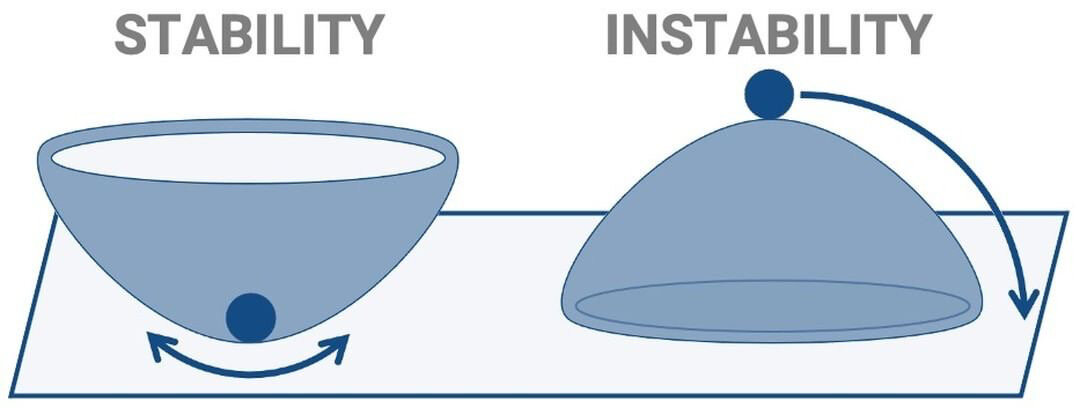
\includegraphics[width=0.7\textwidth]{images/ConceptOfStability.png}
\end{center}
\end{frame}

\begin{frame}[allowframebreaks]{In power systems}
\begin{quote}
    \textbf{Power system stability is the ability of an electric power system, 
    for a given initial operating condition, to regain a state of operating equilibrium 
    after being subjected to a physical disturbance, with most system variables bounded 
    so that practically the entire system remains intact.} \cite{hatziargyriou2020definition}
\end{quote}
\vspace{0.5cm}
\begin{center}
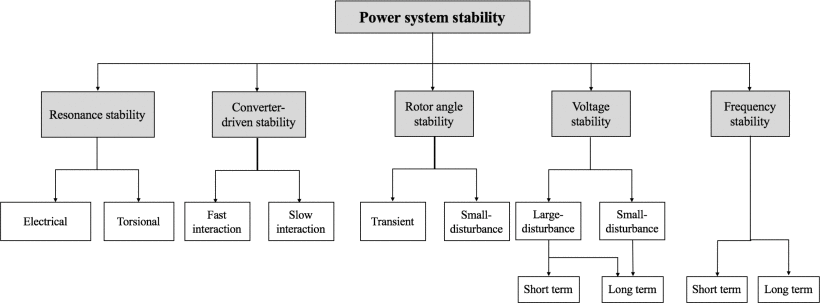
\includegraphics[width=0.9\textwidth]{images/ClassificationStability.png}
\end{center}
\end{frame}


\section{Why do we need stability?}

\begin{frame} {Key points}
\begin{itemize}
    \item We often take electricity as a simple commodity.
    \item But the electric power system is one of the most complex and largest man-made systems.
    \item The chances of system failures are very high taking into account the impact of external factors and rapid changes in the system's state.
    \item However, power systems are very reliable (operated 24h/24h 7d/7d and only a few hours of power outages per year!).
    \item But when instabilities occur, it can lead to blackouts with huge financial and societal consequences.
\end{itemize}
\end{frame}

\begin{frame}{Tokyo 1987}
\begin{columns}
\begin{column}{0.5\textwidth}
    \begin{itemize}
        \item Unexpected load increase and presence of constant power devices (air conditioners) led to a voltage collapse.
        \item \textbf{8 GW lost} and \textbf{2.8M customers impacted} \cite{ohno20061987, kurita1988power}
    \end{itemize}
\end{column}
\begin{column}{0.5\textwidth}
    \begin{center}
    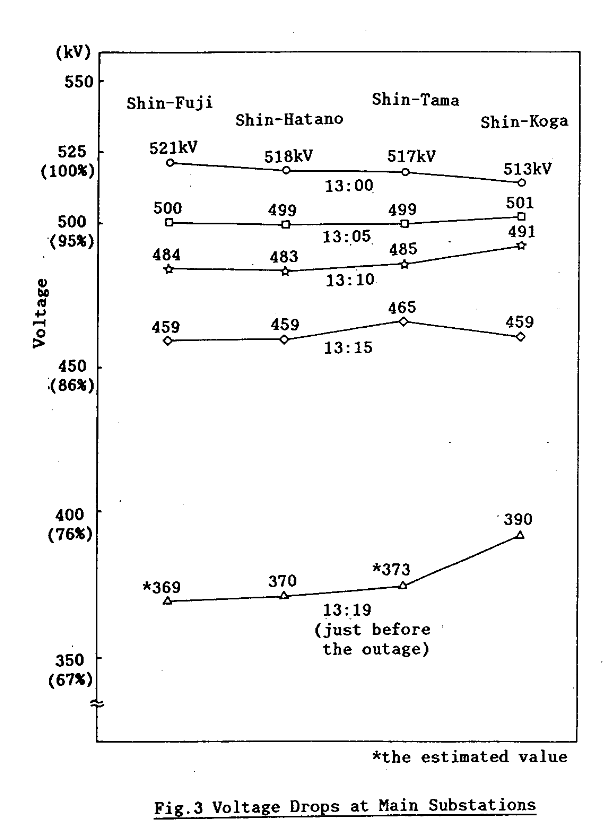
\includegraphics[width=0.7\linewidth]{images/TokyoCollapse.png}
    \end{center}
\end{column}
\end{columns}

\end{frame}

\begin{frame}{Canada/Northeast USA 2003}
\begin{columns}
\begin{column}{0.6\textwidth}
    \begin{itemize}
        \item Initial problem: not enough reactive power reserve. Hot weather and large consumption led to transmission lines overloading and eventually sagging into trees, further deteriorating the initial problem.
        \item A cascading event caused the tripping of hundreds of lines and generating units.
        \item \textbf{63 GW lost} and \textbf{50M customers impacted} and \textbf{Estimated cost above \$5 Billion}
        \item Watch \tiny{\url{https://www.youtube.com/watch?v=nd3teNgUq8E}, \url{https://www.youtube.com/watch?v=KciAzYfXNwU}}
    \end{itemize}
\end{column}
\begin{column}{0.4\textwidth}
    \begin{center}
    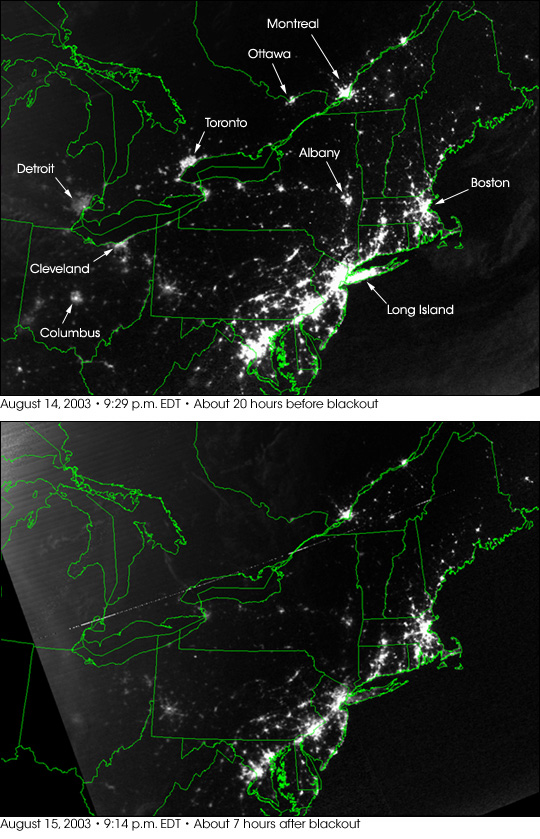
\includegraphics[width=0.6\linewidth]{images/USABlackOut.png}
    \end{center}
\end{column}
\end{columns}


\end{frame}

\begin{frame}[allowframebreaks]{Europe 2006}
\begin{itemize}
    \item Disconnection of a transmission line in Germany for the transport of a ship approved by the local TSO.
    \item The local TSO approved to advance the disconnection later that day, but the commercial flows remained unchanged.
    \item Some lines were critically loaded because of the line disconnection and a fast increase of load consumption led to a cascading event.
    \item The European interconnected network was split into 3 islands.
    \item Watch \url{https://www.youtube.com/watch?v=A30DdnsICuw}
    \item \textbf{14.5 GW lost} and \textbf{15M customers impacted} \cite{li2007analysis}
\end{itemize}

\begin{center}
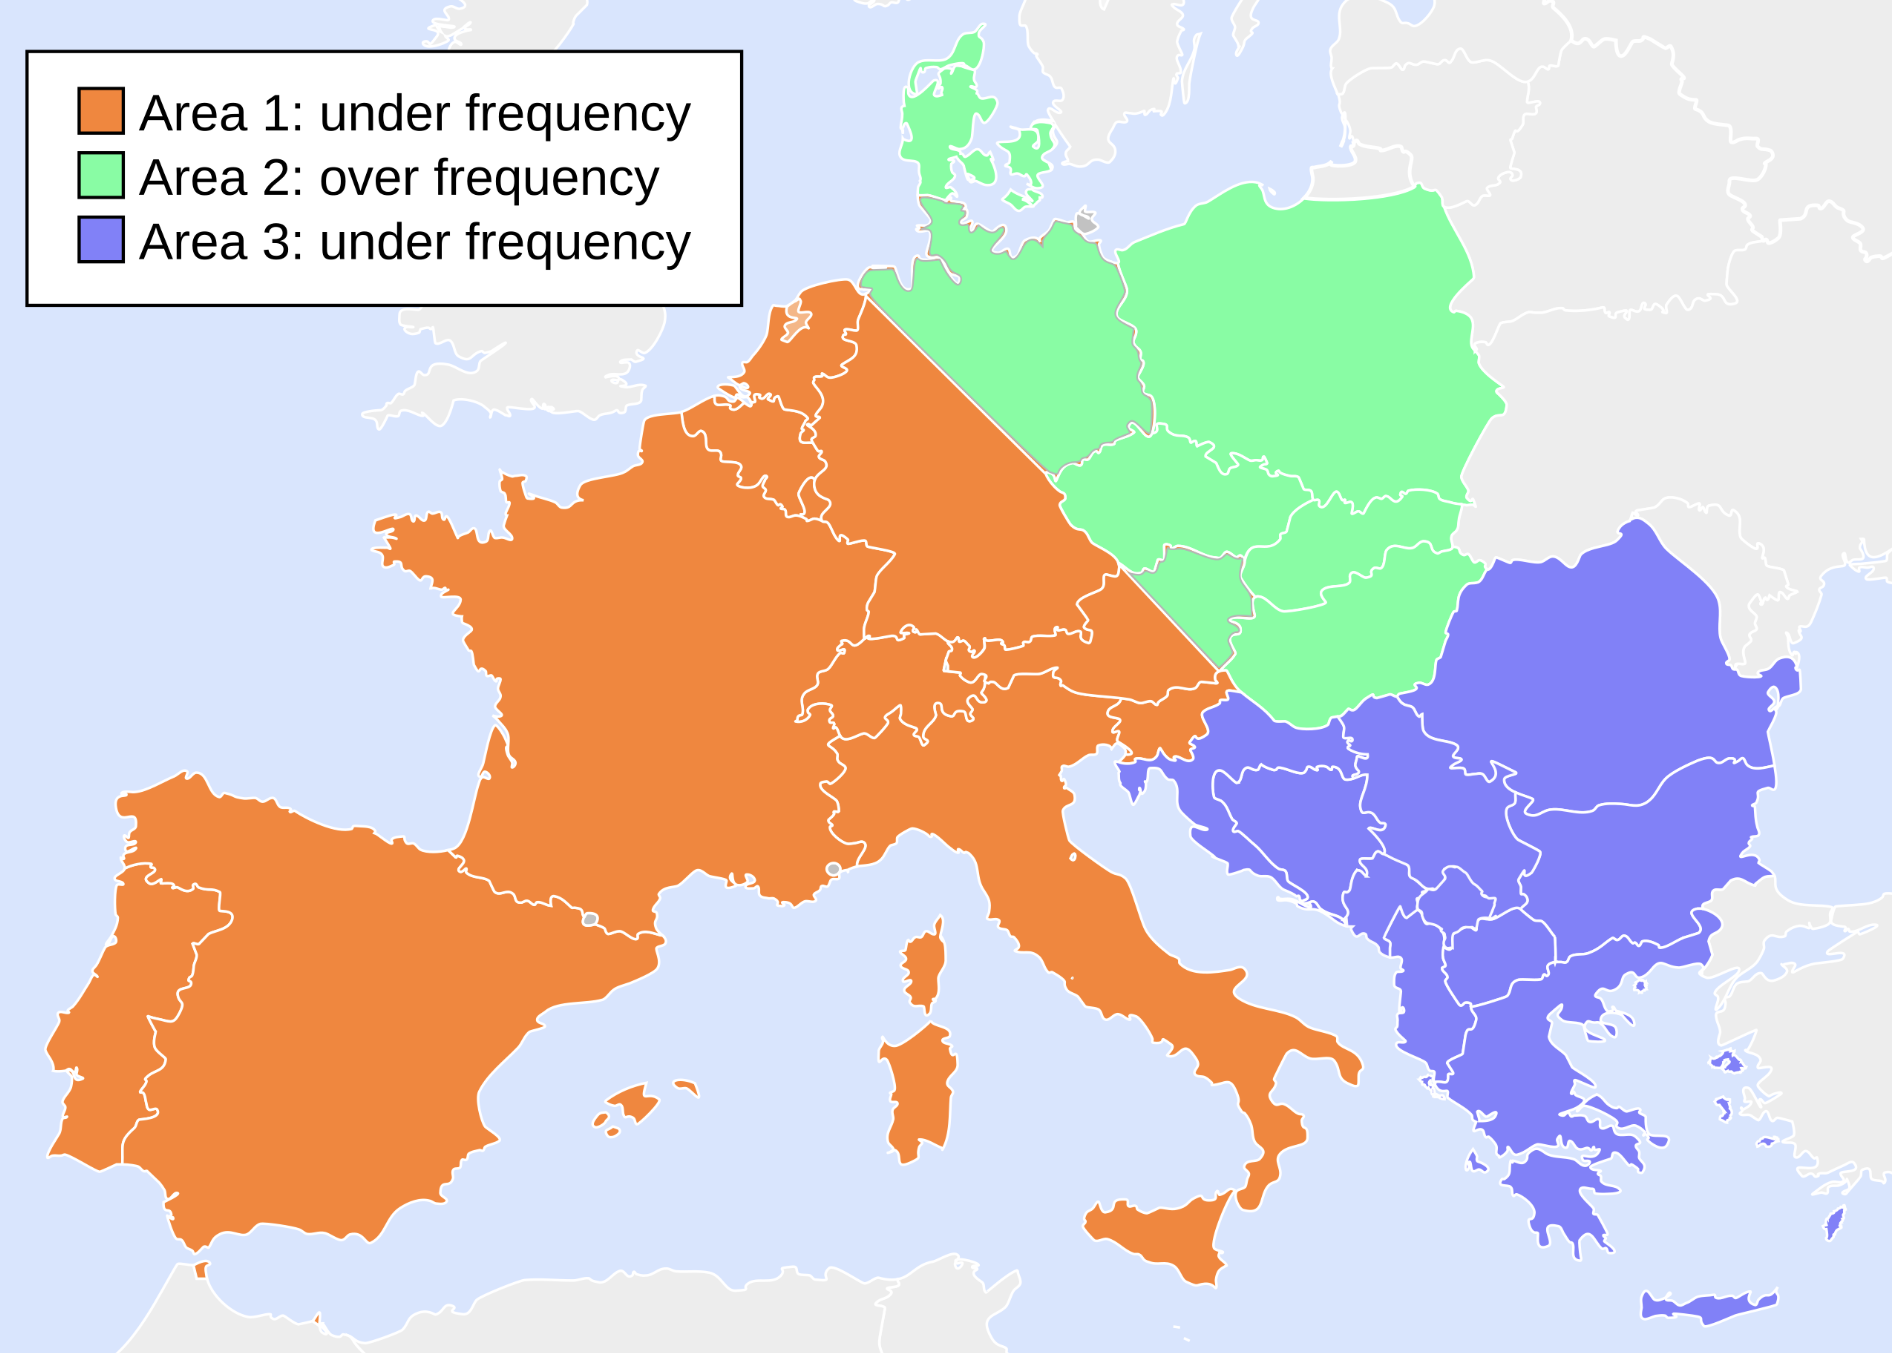
\includegraphics[width=0.6\textwidth]{images/EuropeBlackOut.png}
\end{center}
\end{frame}

\begin{frame}{Brazil 2023}
\begin{itemize}
    \item False operation of a relay protection system led to a 500kV line disconnection.
    \item The Energy Management System did not operate properly.
    \item \textbf{19 GW lost}
\end{itemize}
\end{frame}
\begin{frame}{Conclusion}
\begin{itemize}
    \item Every time a blackout happened, lessons have been learned, and new rules have been put in place.
    \item Nonetheless, due to the system complexity, new complex phenomena occur that power system engineers try to understand.
    \item In the following, we'll dive into the mechanisms of voltage instability.
\end{itemize}
\end{frame}